%%
\chapter{Typesetting Topics}
\label{chapter:typesetting}

This chapter will go through some of the \tex features you'll probably want to use at some point.
So far, {\em most} of the things I usually do with \tex can be made to work for eBook outputs,
but there are lots of commands and options that don't work and you need to know which
variants to use.

%%
\section{References and Citations}

One of the easy things that `just works' most of the time in \latex is references. For example,
the \tex source for this chapter starts with:

\begin{Verbatim}[fontsize=\small]
\chapter{Typesetting Topics}
\label{chapter:typesetting}
\end{Verbatim}

Then if I want to refer to the chapter, I write \sverb|Chapter \ref{chapter:typesetting}| which
gets rendered as `Chapter \ref{chapter:typesetting}'. Adding \smalltt{label} commands for tables and figures
works in the same way.

This isn't rocket science, but if you've ever tried
renumbering by-hand, you know how valuable this is! Similarly, bibliographic references such as
\sverb|\cite{knuth1984texbook}| work correctly, giving a citation looking like \cite{knuth1984texbook}.
So far \textsc{BibTeX} has worked fine for this book.

%%
\section{Graphics}

Nearly all eBooks have graphics in them somewhere, even if just for a cover page. 
The \smalltt{graphicx} package works well for this.
For example, the cover image for the title page of this book is included using the command:

\begin{Verbatim}[fontsize=\small]
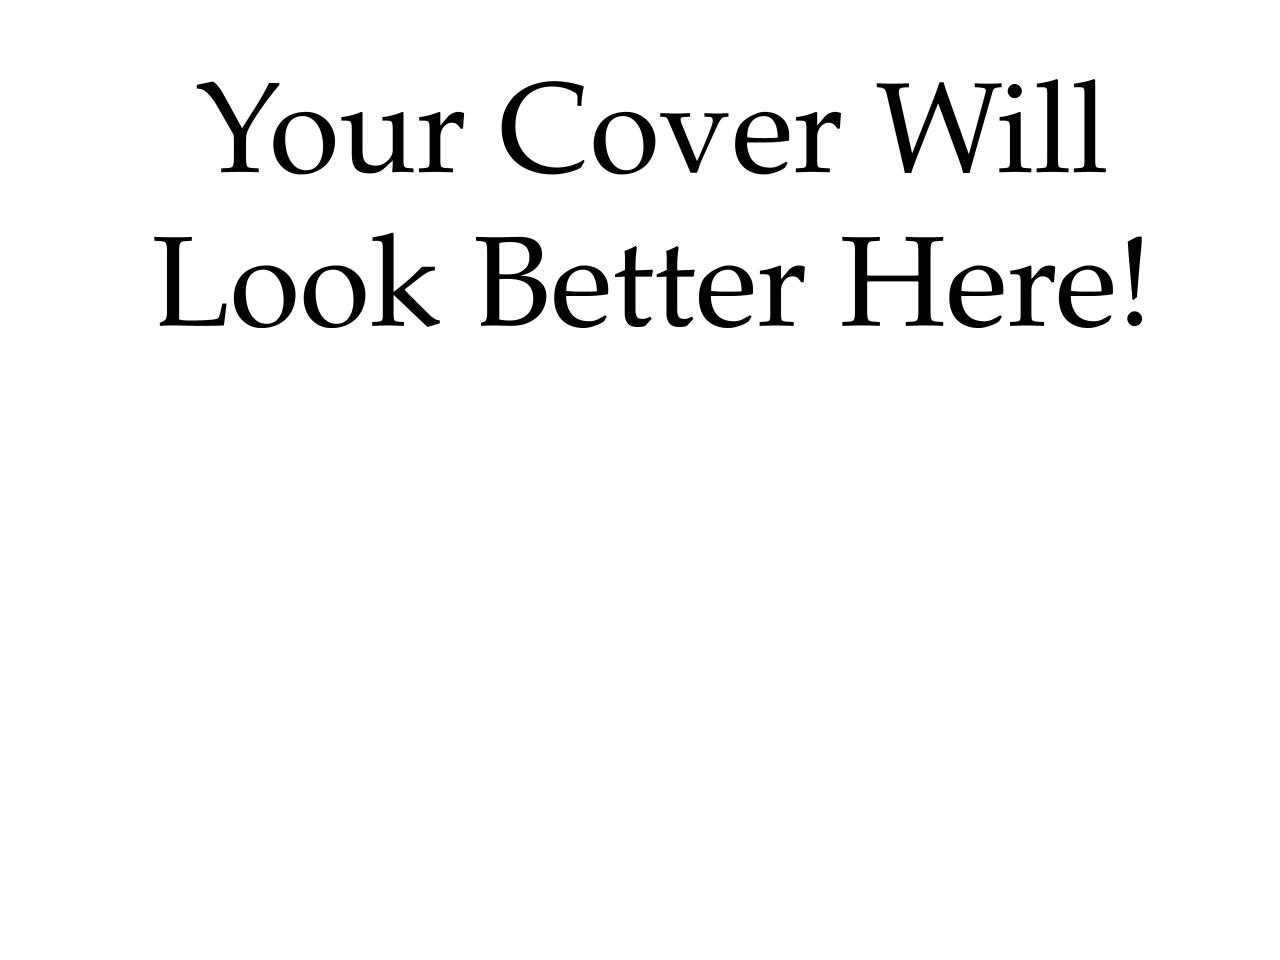
\includegraphics[width=0.8\linewidth]{images/cover.png}
\end{Verbatim}

Typically for webpages and eBooks, the size of images is expected to vary with the page size and settings,
so using a context-sensitive width like a proportion of the linewidth is more appropriate than a fixed-width
declaration like `10cm'. Many eReaders enable users to click on images to see them in more detail, which helps.

One frequent problem is that HTML typesetting using \smalltt{htlatex} or a similar process doesn't always preserve the
aspect ratio of your images. For example, the same setting may be used for width and height, making all images square.
The problem is solved by adding a bounding box file using the \smalltt{extractbb} command, which is typically included
with \tex distributions. For this book, this step is included in the project's \smalltt{build.sh} script, at least for \smalltt{.jpg} and
\smalltt{.png} files, and it can easily be extended to more filetypes. Or you can run \smalltt{extractbb -x \$IMAGE} on these files
yourself.

Images are often put in the \latex \smalltt{figure} environment, which can include captions and a label for references.
For example, the map in Figure \ref{fig:sea_map} is created using the commands:

\begin{Verbatim}[fontsize=\footnotesize]
\begin{figure}
\begin{center}
  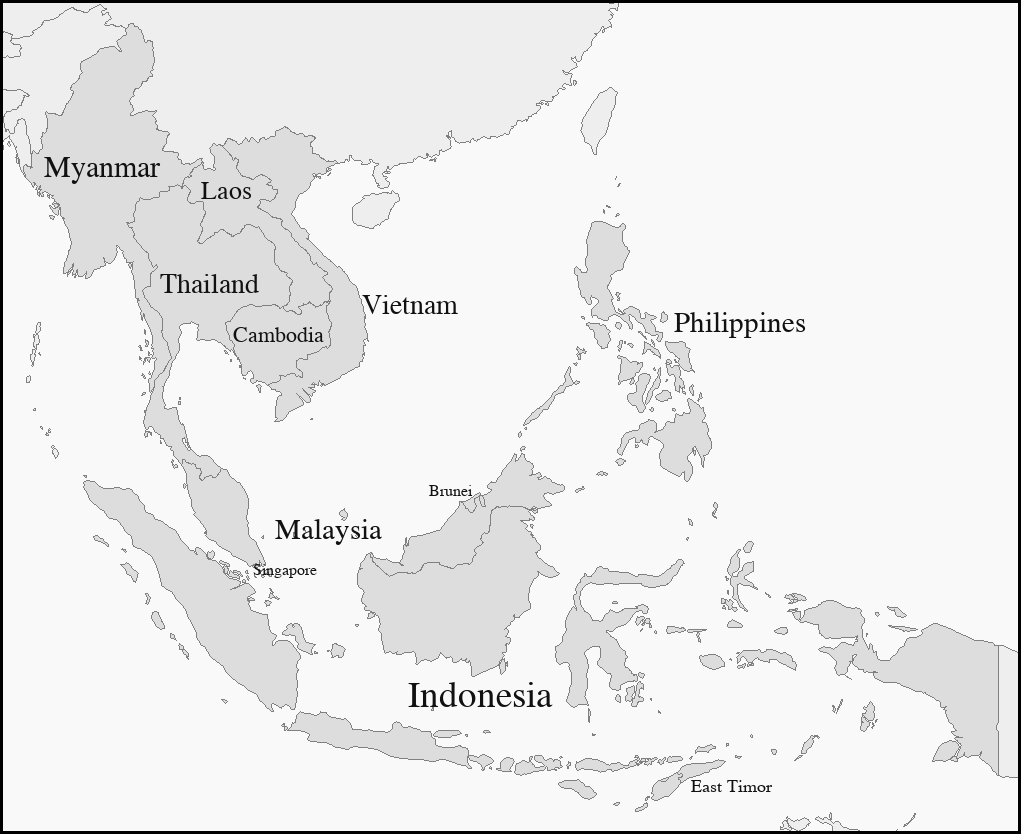
\includegraphics[width=1.2\linewidth]{images/sea_countries.png}
  \caption{Map of countries in Southeast Asia}
  \label{fig:sea_map}
\end{center}
\end{figure}
\end{Verbatim}
  
\begin{figure}
\begin{center}
  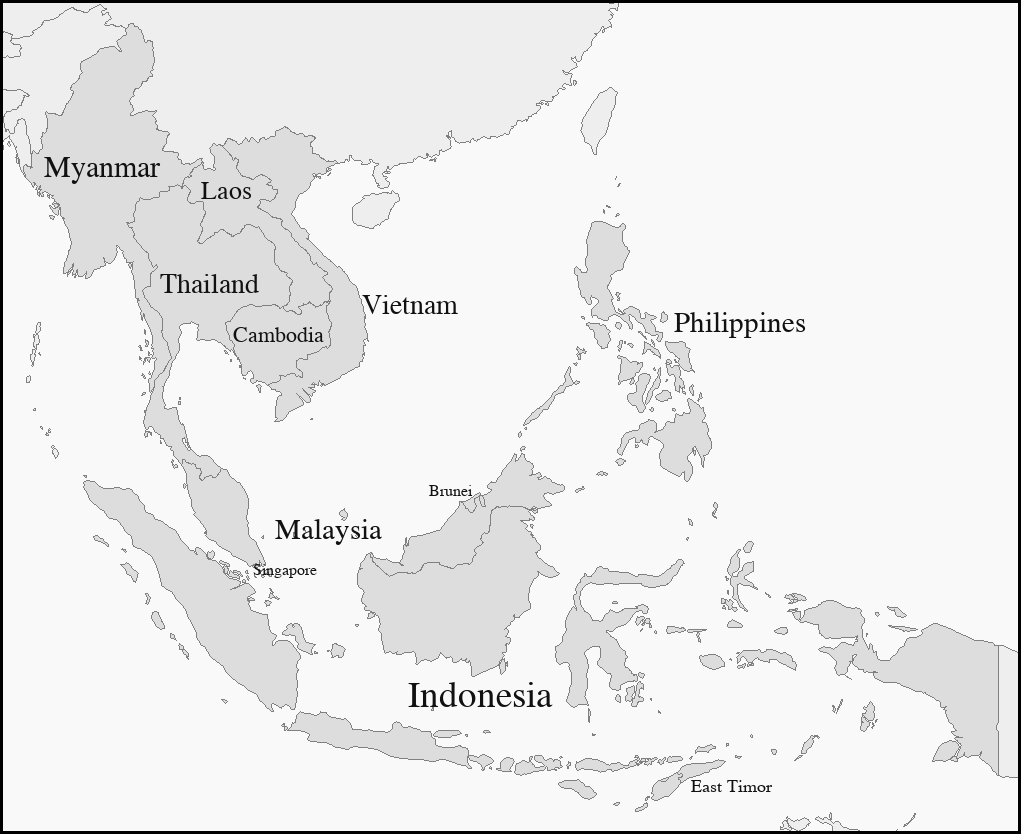
\includegraphics[width=1.2\linewidth]{images/sea_countries.png}
  \caption{Map of countries in Southeast Asia}
  \label{fig:sea_map}
\end{center}
\end{figure}

From here, the figure can be referenced using the command 
\sverb|\ref{fig:sea_map}|. (Made using \surl{https://github.com/dwiddows/pilmaps},
a free mapping tool in python that supports low-level, hands-on rendering control --- feel free to try it out.) 
So far I haven't found an effective way of controlling the placement of figures --- for example, directives
like \sverb|\begin[ht]{figure}| don't affect the HTML or the ePub output, and I haven't got
wraparound text to work.

 %%
\section{Tables}

Basic tables typeset just fine in \smalltt{epub} format. They don't format properly in the Kindle preview of \smalltt{mobi} files,
and I'm hoping that this won't affect the end result on Kindle \smalltt{epub}  books downloaded form the store.

For example, the following \latex gives the output in Table \ref{tab:artist_works}.

\begin{Verbatim}[fontsize=\footnotesize]
\begin{table}
  \centering
  \begin{tabular}{|c|l|}
    \hline
    \textbf{Artist} & \textbf{Great Works} \\
    \hline
    Leonardo da Vinci & The Mona Lisa \\
    Charlie Watts & Satisfaction \\
    \hline
  \end{tabular}
  \caption{Inspiring works}
  \label{tab:artist_works}
\end{table}
\end{Verbatim}

\begin{table}
 \centering
  \begin{tabular}{|c|l|}
    \hline
    \textbf{Artist} & \textbf{Great Works} \\
    \hline
    Leonardo da Vinci & The Mona Lisa \\
    Charlie Watts & Satisfaction \\
    \hline
  \end{tabular}
  \caption{Inspiring works}
  \label{tab:artist_works}
\end{table}

With standard \latex it is easy to make tables that are too big for pages or that typeset poorly for other of reasons.
I expect this can be even more of a problem with small-screen eBooks, so you'll want to design any tables accordingly
and check output carefully.

%%
\section{Equations}

One of the benefits of \latex is that it's easy to typeset mathematical notation like formulae and equations. So far these look to work well in HTML and eBook formats.

For example, here is the \tex and its rendering for Euler's formula:

\begin{Verbatim}[fontsize=\scriptsize]
\[ e^{ix} = \cos x + i \sin x \]
\end{Verbatim}
\[ e^{i\pi} = -1 \]

And here is the corresponding \tex and output for a Fourier series:

\begin{Verbatim}[fontsize=\scriptsize]
\[ f(x) = \sum_{k=0}^{\infty} [  a_k \sin(kx) + b_k \cos(kx) ] \]
\end{Verbatim}
\[ f(x) = \sum_{k=0}^{\infty} [  a_k \sin(kx) + b_k \cos(kx) ] \]

Array environments for typesetting rows and columns in equations also work, for example:

\[
u = \left( \begin{array}{c} 1 \\ 0 \\ -2 \end{array} \right) \qquad
v = \left( \begin{array}{c} 2 \\ -1 \\ 3 \end{array} \right) \qquad
u^T v = 2 + 0 - 6 = -4 \qquad
u v^T = \left( \begin{array}{ccc} 2 & -1 & 3 \\ 0 & 0 & 0 \\ -4 & 2 & -6 \end{array} \right)
\]

This set of equations may become typeset in a smaller font than those above, to fit them
horizontally on a small screen. If these start to get too small, consider breaking lines up
when typesetting mathematics for eBooks.

%%
\section{Contents and Index}

The table of contents should get typeset entirely automatically if you use this template.

The story of how traditional indexes and concordances influenced the design of the inverted
indexes used by search engines is fascinating \citep[Ch 1]{witten1999gigabytes}.
By now, for electronic books, this process is quite complete: the index is created automatically,
and accessed via the search interface, not by the user scrolling through topics in alphabetical order.
If you want to make a paper
version of your book as well as an eBook, you may want to reconsider this.

If you do want to make a paper book as well, it may be worth trying a
more sophisticated template such as the one that comes with Clemens
Lode's book on using \latex for books and eBooks \citep{lode2019better}.
This includes conditional compilation so that different commands and even sections are used
for the PDF version that leads to a paper book and the HTML version that leads to an eBook.

%%
\section{Difficulties}

Several things are hard and may just not work with typesetting to HTML.

Exact placement is sometimes impossible. Figures, tables, and captions may appear
in various places, and often don't obey typesetting directives. For example,
putting an \sverb|fbox| (framebox) around a figure makes it float to the left, irrespective of
centering commands. Captions may easily fall across
a page boundary, so one tip is to keep captions small (one line), just enough for the reader
of the main text to see that they are looking at the right table or image.

Controlling font size in different environments has been hard, particularly with typewriter fonts
used for verbatim text such as rendering \latex commands that you don't want to be interpreted as
\latex commands. In retrospect, trying to write an eBook about \latex itself was perhaps not the
most sensible decision! But this has been fixed using the right combination of commands from the
\sverb|fancyvrb| package, included here as macros like \sverb|\sverb| for `small verbatim' and
\sverb|\surl| for `small URL'.

Some of these things lead to important design considerations.
Remember that we're designing for a small screen, whose font size and spacing is up to the user. 
There no point making a particular page (say page 33) look perfect on your device,
only to be reminded that for someone with a larger font setting, this could be spread across
pages 44 and 45. Don't get too ambitious with making your book
look `just right' on one device --- instead, once something is clear and legible, be thankful
that it can reach so many varied users.

